

In this paper we aim to get a better understanding of the unstable logs in an application so that we can improve the maintenance of log processing tools. In this section we present our rationale for selecting the applications we studied and present our data extraction and analysis approach.

\subsection{Subject systems}
We evaluate our approach through a case study on four open source applications. We select these projects on the following two criteria:
\begin{itemize}
	\item \textbf{Log usage -} We select applications that make use of extensive logging in their source code. 
%	This helps to improve the performace of the random forest classifier and to identify the factors which effect log stability.
	\item \textbf{Project activity -} We pick applications which have a large user base and commit history to identify and track the log changes across multiple releases. 
\end{itemize}

To find the number of logs present in an application we `grep' to search all lines of code within the `.java' files. Next, using git log we find the total number of commits in the open source projects and pick ones which have more than 10,000 commits. We find four open source projects from the Apache git repository which fit these criteria: ActiveMQ, Camel, CloudStack  and Liferay. Table~\ref{tba:overviewsystems} presents an overview of the applications.


% which had more than 10,000 commits. We also verify if the projects utilize a bug tracking system like 'JIRA' or `Bugzilla' because, this helps to tag commits to specific development activities (i.e., bug fix, improvement, new-features). We use the `grep' command to recursively search for all log lines within `.java' files in the latest release of each project in the cloned repositories. The four open source projects are: Liferay, Camel, ActiveMQ and CloudStack. All studied systems have extensive system logs and Table~\ref{tba:overviewsystems} presents an overview of the systems.

\textbf{ActiveMQ}\footnote[1]{http://activemq.apache.org/} is an open source message broker and integration patterns server.

% We covered ActiveMQ release 4.1.1 to 5.9.0 which cover more than 6 years of development from 2007 to 2013.

\textbf{Camel}\footnote[2]{http://camel.apache.org/} is an open source integration platform based on enterprise integration patterns. We analyze Camel release 1.6 to 2.11.3 which cover more than five years of development from 2009 to 2013. 

\begin{table}[tbh]
	\centering \protect\protect\caption{An overview of all studied applications}
	
	
	\label{tba:overviewsystems} %
	\begin{tabular}{lllll}
		\hline 
		Projects  & ActiveMQ  & Camel  & CloudStack  & Liferay \tabularnewline
		\hline 
		Starting release  & 4.1.1  & 1.6.0  & 2.1.3  & 6.1.0-b3 \tabularnewline
		End release  & 5.9.0  & 2.11.3  & 4.2.0  & 7.0.0-m3 \tabularnewline
		Total \# log lines  & 5.1k  & 6.1k  & 9.6k  & 1.8k \tabularnewline
		Total \# of releases  & 19  & 43  & 111  & 24 \tabularnewline
		Total added code  & 261k  & 505k  & 1.09M  & 3.9M \tabularnewline
		Total deleted code  & 114k  & 174k  & 750K  & 2.8M \tabularnewline
		Total \# added logs  & 4.5k  & 5.1k  & 24k  & 10.4k \tabularnewline
		Total \# deleted logs  & 2.3k  & 2.4k  & 17k  & 8.1k \tabularnewline
		\hline 
	\end{tabular}
\end{table}


\textbf{CloudStack}\footnote[3]{https://cloudstack.apache.org/} is open source software designed to deploy and manage large networks of virtual machines. 
%as a highly available, highly scalable Infrastructure-as-a-Service (IaaS) cloud computing platform. We covered CloudStack release 2.1.3 to 4.20 which cover more than 3 year of development from 2010 to 2014.


\textbf{Liferay}\footnote[4]{http://www.liferay.com/} is an open source software to deploy websites and portals. 

% is a free and open source enterprise project written in Java. It provides platform features which are used in development of websites and portals. We study the releases from 6.1.0 to 7.0.0-m3 which cover more than three years of development from 2010 to 2014
% We select liferay as it is one of the leading platforms for platform development~\cite{LiferayGartner} and has growing user base~\cite{LiferayUser}.
%  It also has an extensive issue tracking system in JIRA which helps in categorizing the commits as bug fixes, improvements, .
  
 

%Hadoop is an open source software framework for distributed storage and for the processing of big data on clusters. Hadoop uses the MapReduce data-processing paradigm. The logging characteristics of Hadoop have been studied in prior research~\cite{IanWCRE,EMSEIAN,IanContextinformation}. We study the releases from Hadoop 0.20.1 to 2.2.0.






Figure~\ref{fig:LGmethod} shows a general overview of our approach, which consists of five steps: (1) We mine the git repository of each studied application to extract all commits made for each file.(2) We identify the log changes in the extracted files. (3) We track the changes made to each log across the commits. (4) We categorize the log changes in the commit and collect the process and change metrics for each log change in the commit 5) We build a random forest classifier and find important metrics which help in understanding the stability of log changes.  We use a statistical tool R~\cite{ihaka1996r}, to perform experiments on the data to answer our research questions. 

\begin{figure}[th]
	\centering
	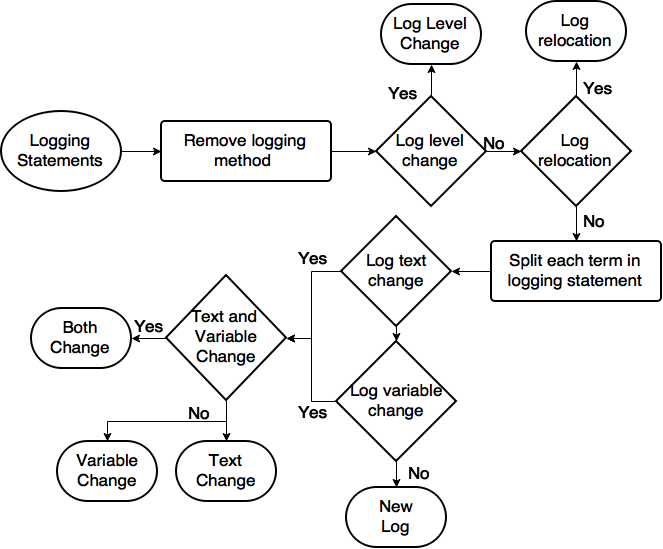
\includegraphics[width=0.7\linewidth]{Flowchart2}
	\caption{Flowchart to categorize the different types of log changes that occur}
	\label{fig:Flowchart2}
\end{figure}

\subsection{Study Approach}

 In the reminder of this section we describe the first four of these steps in detail and the explain the construction of random forest classifier in Section~\ref{prediction}.

\subsubsection{Extracting the change history }
In order to find the stability of logs we have to identify all the `Java' files in our studied applications. To achieve this, we clone the \emph{master} branch of the git repository of each studied application locally. We use the `find' command to recursively find all the files which end with pattern `*.java'. To remove the \textsl{Java Test} files, we use the `grep' command to filter all files which have `test' or `Test' in their pathname.

 After collecting all the Java files from the four studied applications, we use the respective git repositories to obtain all the changes made to the file within the time-frame discussed above. We use the `follow' option to track the file even when they are renamed or relocated within our studied applications. We also flatten all the changes made to files to include the changes made in different branches but exclude the final merging commit. Using this approach, we obtain a complete history of each \emph{Java} file in the latest version of the master branch.

\subsubsection{Identifying Log Changes}
From the extracted change history of each \emph{Java} file, we identify all the log changes made in the commits. To identify the log statements in the source code, we manually sample some commits from each studied application and identify the logging library used to generate the logs. We find that the studied applications use \textsl{Log4j}~\cite{EMSEIAN} and \textsl{Slf4j}\footnote{http://www.slf4j.org/} widely and \textsl{logback}\footnote{http://logback.qos.ch/} sparingly. Using this information, we identify the common method invocations that invoke the logging library. For example, in  ActiveMQ and Camel a logging library is invoked by method named `LOG' as shown below.
\hypobox{ LOG.debug(``Exception detail", exception);}

%In CloudStack it is usually done through `\_logger' as follows.
%
%\hypobox{\_logger.warn(``Timed out: " + buildCommandLine(command));}

As a project can have multiple logging libraries throughout its life-cycle, we use regular expressions to match all the common log invocation patterns (i.e., `LOG',`log',`\_logger',`LOGGER',`Log'). We count every invocation of a logging library followed by a logging level (`info', `trace', `debug', `error', `warn') as a log.

%We count every such invocation of alogging library as a log.


\subsubsection{Tracking Log Changes}
After identifying all the log changes made to a file across multiple commits, we track each log individually to find out whether it has changed in subsequent revisions. We first collect all the logs present in a file at the first commit, which form the initial set of logs for the file. Every subsequent commit which has changes to a log appears as an added and deleted log in \textsl{git}. To track these log changes made, we used the Levenshtein ratio~\cite{levenshteinratio}. We use Levenshtein ratio instead of string comparison, because Levenshtein ratio quantifies the size of difference between the strings compared within the range 0 to 1 (more similar the strings the ratio approaches 1). 

%To calculate Levenshtein ratio for a pair of added and deleted logs, we first remove the logging method (e.g., LOG) and compare the remaining text to increase the accuracy of categorization. 


%We set a minimum threshold of 0.6 for a pair of added and deleted logs to be considered modified. We set 0.6 because there is atleast 60\% similarity between the pair. We find that when the threshold is set lower there are more false positives and when set higher we miss log modifications. When an added log has levenshtein ratio higher than 0.6 with multiple deleted logs, we consider the pair with highest levenshtein ratio. 
We calculate the Levenshtein ratio for each deleted log against all the added logs and pick the pair which has the highest Levenshtein ratio  as a modification. This is done recursively to find all the modifications within a commit. For example in the logs shown below, we find that the Levenshtein ratio between the added and deleted pair (a1) is 0.86 and (a2) 0.76. Hence, we consider (a1) as a log modification.  
 \hypobox{-        LOG.debug(``Call: " +method.getName()+ `` " + callTime);\\
 +      LOG.debug(``Call: " +method.getName()+`` took "+ callTime + ``ms"); \space  \space  \space  \space  \space  \space -- (a1)\\ 
 +      LOG.debug(``Call: " +method.setName()+`` took "+ callTime + ``ms");\space  \space  \space  \space  \space  \space -- (a2)\\} 


If the added log does not match any log in our initial set, it is considered as a new log addition and is added to the initial set for tracking in future commits. From this we can track how many times a log is changed and how many commits are made between the changes. 


%\subsubsection{Match JIRA to Log Changes}



\subsubsection{Categorize log changes}

When logs are changed, they can be changed in four possible ways namely:
\begin{enumerate}
	
	\item { \textbf{Log relocation:} } The log is kept intact but moved to a different location in the file because of context changes (code around the log is changed).
	
	\item \textbf{Text change:} The text (i.e., static content) of log is changed. 
	
	\item\textbf{Variable change:} One or more variables in the log are changed (added, deleted or modified).
	
	\item \textbf{Change of log level:} The verbosity level of a log is changed.
	
%	\item  \textbf{Text and variable change:} Both text and variables in the logs are changed. This is generally done when developers provide more context information, i.e, text and add/modify the relevant variables in a log.
	
\end{enumerate}


To automate the process of categorizing log changes into these categories, we first remove the logging method (i.e, LOG) and the log level (i.e, info) from the logs. We then compute the \textsl{Levenshtein ratio} between each term within the parentheses. In the example below we find that `+ Integer.toString(listenPort)' has \textsl{Levenshtein ratio} of 1, implying they are identical and the \textsl{Levenshtein ratio} between `starting HBase HsHA Thrift server on' and `starting HBase' is 0.56. This suggests there is some similarity between the two strings and the variable is constant which implies its a text change. Figure~\ref{fig:Flowchart2} highlights the process of categorizing the log changes.

\hypobox {+ LOG.info(``starting HBase HsHA Thrift server on " + Integer.toString(listenPort)); }

\hypobox {- LOG.info(``starting HBase " + Integer.toString(listenPort)); }


%Using the commit data, we also track the JIRA issues to extract the developer metrics such as developer experience, number of developers involved, issue priority. To achieve this, we extract the JIRA issue IDs from commit messages and use the JIRA repository to extract the JIRA issue. The JIRA issue contains information about the issue such as, type (i.e., bug, improvement, new-feature, task), priority, resolution time and developer information such as number of comments and number of developers involved in the JIRA discussion. We use this information along with code and log churn metrics for answering our research questions. 




 







